\documentclass[10pt]{beamer}

\usetheme[sectionpage=none, progressbar=frametitle]{metropolis}

\definecolor{alertblue}{RGB}{0,110,191}
\definecolor{DarkGray}{RGB}{51,51,51}
\definecolor{RedAlert}{RGB}{255,0,0}

\setbeamercolor{progress bar}{fg=alertblue,bg=fg!50!black!30}
\setbeamercolor{normal text}{fg=DarkGray}
\setbeamercolor{alerted text}{fg=RedAlert}

%% =============================================================================
%%
%%                                      PACOTES
%%
%% =============================================================================

\usepackage[utf8]{inputenc}
\usepackage[brazil]{babel}
\usepackage{booktabs}
\usepackage[scale=2]{ccicons}
\usepackage{pgfplots}
\usepgfplotslibrary{dateplot}
\usepackage{xspace}
\usepackage{amsmath}
\usepackage{tikz}
\usepackage{multirow}
\usepackage{upgreek}
\usetikzlibrary{calc}
\usepackage[
type={CC},
modifier={by-nc-sa},
version={4.0},
]{doclicense}
\newcommand{\themename}{\textbf{\textsc{metropolis}}\xspace}


%% =============================================================================
%%
%%                                      INFOS
%%
%% =============================================================================


\title{Fundamentos de Escoamentos Reativos Turbulentos}
\subtitle{Aula 2-3}
\date{28 de setembro de 2020}
\author{Prof. Dr. Guenther Carlos Krieger Filho}
\institute{Escola Politécnica da USP - LETE/CRC - Combustion Research Centre}
\titlegraphic{
\includegraphics[height=1.0cm]{Logo-LETE_1.png}\hfill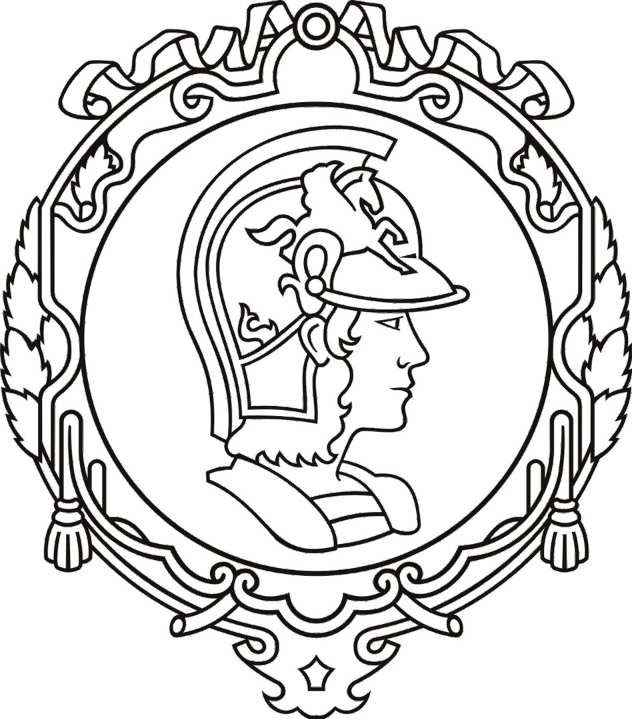
\includegraphics[height=1.5cm]{logo.png}}

%================================ USER DEFINED ==================================

\newcommand{\ddt}[1]{\dfrac{\partial #1}{\partial t}}
\newcommand{\tgrad}[1]{\dfrac{\partial #1}{\partial x_j}}
\newcommand{\ddx}[2]{\dfrac{\partial #1}{\partial x_{#2}}}
\newcommand{\ddxp}[2]{\dfrac{\partial }{\partial x_{#2}}\left(#1\right)}
\newcommand{\laplace}[1]{\dfrac{\partial^2 #1}{\partial x_{j}\partial x_{j}}}
\newcommand{\m}[1]{\overline{#1}}
\newcommand{\divr}[1]{\nabla \cdot #1}
\newcommand{\divp}[1]{\nabla \cdot \left(#1\right)}
\newcommand{\red}[1]{{\color{red}#1}}
\newcommand{\blue}[1]{{\color{blue}#1}}
\newcommand{\incircle}[1]{{\tikz[baseline=(X.base)] \node(X)[draw, shape=circle, inner sep=0]{\strut #1};}}
%=========================================              =========================================
\metroset{block=fill}
\begin{document}

%% =============================================================================
%%
%%                                      TITULO
%%
%% =============================================================================
\maketitle

%\begin{frame}{Conteudo}
%  \setbeamertemplate{section in toc}[sections numbered]
%  \tableofcontents[hideallsubsections]
%\end{frame}

\section{Introduction}

\begin{frame}[fragile]{Descrição de escoamentos turbulentos}
	%\metroset{block=fill}
	\begin{columns}
		\column{0.5\textwidth}
		\begin{figure}
			\centering
			%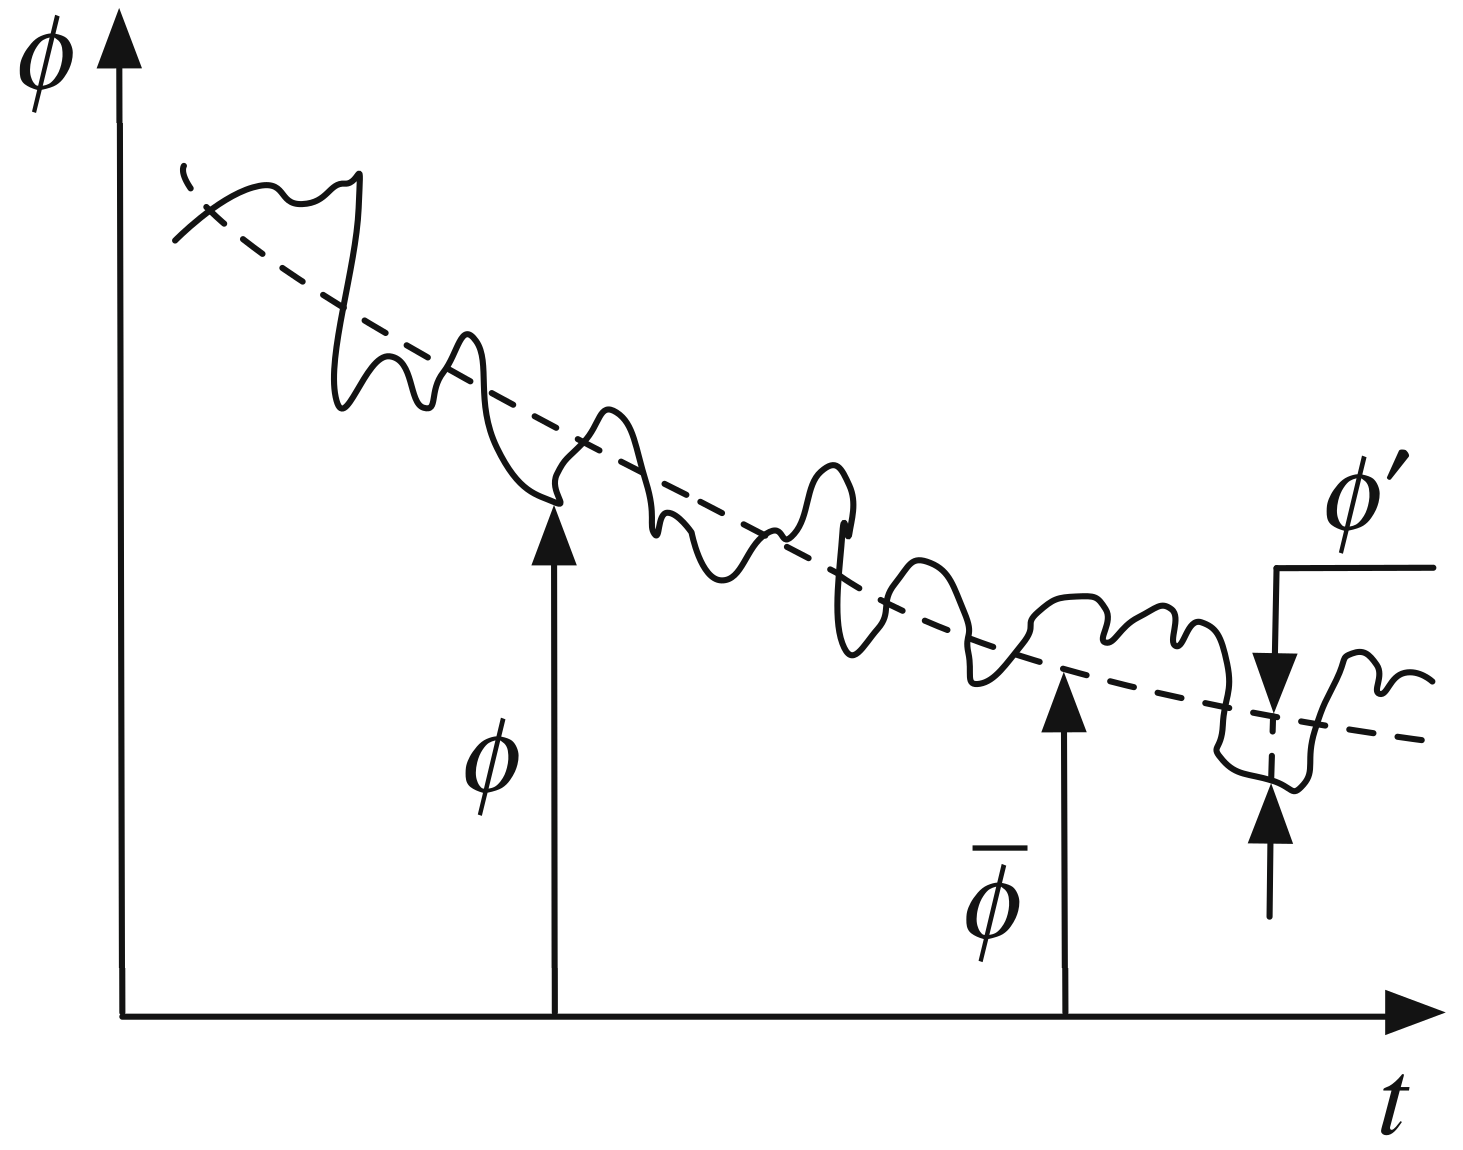
\includegraphics[width=0.8\linewidth]{phixtime}
			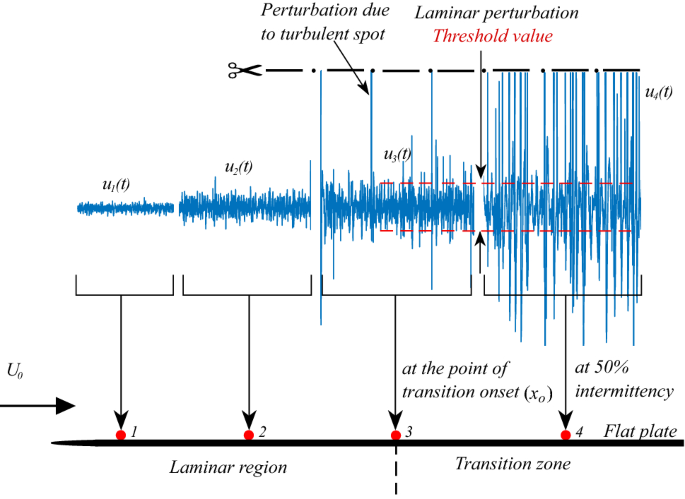
\includegraphics[width=0.8\linewidth]{velFluct}
			\label{fig:velFluct}
		\end{figure}
	\begin{block}{Média no tempo}
		\begin{equation*}
		\m{\Phi} = \dfrac{1}{\Delta t} \int_{0}^{\Delta t} \Phi_{(t)} dt
		\end{equation*}
	\end{block}
	
		\column{0.5\textwidth}
		\begin{block}{Ergodicidade}
			\centering
			Média conjunto = Média no tempo
			
			(Média estatística)
		\end{block}
	
		\begin{block}{Decomposição de Reynolds}
			\begin{equation*}
			\Phi_{(t)} = \m{\Phi} + \Phi'_{(t)}
			\end{equation*}
		\end{block}
	\end{columns}
	
	\begin{align*}
	\dfrac{1}{\Delta t} \int_{0}^{\Delta t} \Phi_{(t)} dt
	&= \dfrac{1}{\Delta t} \int_{0}^{\Delta t} \m{\Phi} dt
	+ \dfrac{1}{\Delta t} \int_{0}^{\Delta t} \Phi' dt \\
	\m{\Phi} &= \m{\Phi} + \m{\Phi'} \rightarrow \boxed{\m{\Phi'} = 0}
	\end{align*}

\end{frame}


\begin{frame}[fragile]{Descrição de escoamentos turbulentos}
	%\metroset{block=fill}
	\begin{columns}
		\column{0.5\textwidth}
		\begin{block}{Variância}
			\begin{equation*}
			\m{(\Phi')^2} = \dfrac{1}{\Delta t} \int_{0}^{\Delta t} (\Phi')^2 dt
			\end{equation*}
		\end{block}
		\begin{block}{RMS/Desvio Padrão}
			\begin{equation*}
			\Phi_{RMS} = \sqrt{\m{(\Phi')^2}}
			\end{equation*}
		\end{block}
		\column{0.5\textwidth}
		\begin{block}{Energia Cinética Turbulenta}
			\begin{equation*}
			K = \dfrac{1}{2} \left[ \m{(u')^2} + \m{(v')^2} + \m{(w')^2} \right]
			\end{equation*}
		\end{block}
		
		\begin{block}{Intensidade Turbulenta}
			\begin{equation*}
			I = \dfrac{\left(\frac{2}{3} K \right)^{1/2}}{U_{\text{ref}}}
			\end{equation*}
		\end{block}
	\end{columns}

\end{frame}

\begin{frame}{Momentos (2\textordfeminine ordem) de 2 variáveis}
	\begin{equation*}
	\Phi = \m{\Phi} + \Phi' \;;\;
	\Psi = \m{\Psi} + \Psi' \;;\;
	\m{\Phi'} = \m{\Psi'} = 0 \;;\;
	\boxed{\m{\Phi' \Psi'} = \dfrac{1}{\Delta t} \int_{0}^{\Delta t} \Phi' \Psi' dt}
	\end{equation*}
	\begin{equation*}
		\text{Para velocidade: }\begin{cases}
		 & u'v' \\ 
		 & u'w'  \\ 
		 & v'w' \\ 
		\end{cases} \text{ Se = 0 }\Rightarrow \text{grandezas não correlacionadas}
	\end{equation*}
	%\metroset{block=fill}
	\begin{block}{Autocorrelação temporal}
		\begin{equation*}
		R_{\Phi'\Phi'(\uptau)} = \m{\Phi'_{(t)}\Phi'_{(t+\uptau)}} = \dfrac{1}{\Delta t} \int_{0}^{\Delta t} \Phi'_{(t)}\Phi'_{(t+\uptau)} dt
		\end{equation*}
	\end{block}
	\begin{block}{Autocorrelação espacial}
		\begin{equation*}
		R_{\Phi'\Phi'(\uptau)} = \m{\Phi'_{(t)}\Phi'_{(t+\uptau)}} = \dfrac{1}{\Delta t} \int_{0}^{\Delta t} \Phi'_{(t)}\Phi'_{(t+\uptau)} dt
		\end{equation*}
	\end{block}

\end{frame}

\begin{frame}{Reynolds Averaged Navier Stokes}
	%\metroset{block=fill}
	\begin{block}{Lembrando...}
	\begin{equation*}
	\rho = cte \;;\;\text{decomposição de Reynolds: }\Phi_{(t)} = \m{\Phi} + \Phi'_{(t)}
	\end{equation*}
	\end{block}

	\begin{enumerate}[$\bullet$]
		\item $ \m{\dfrac{\partial \Phi}{\partial s}} 
		\equiv \dfrac{1}{\Delta t} \int_{0}^{\Delta t} \dfrac{\partial \Phi}{\partial s} dt 
		= \dfrac{\partial \m{\Phi}}{\partial s} $
		\vspace*{0.4cm}
		\item $ \m{\int\Phi ds} = \int \m{\Phi} ds $ \vspace*{0.4cm}
		\item $ \m{\Phi + \Psi} = \m{\Phi} + \m{\Psi} $ \vspace*{0.4cm}
		\item $ \m{\Phi \Psi} = \m{(\m{\Phi} + \Phi') (\m{\Psi} + \Psi')}
		= \m{\m{\Phi}\;\m{\Psi}} + \m{\Phi'\Psi'}
		+ \underbrace{\m{\m{\Phi}\Psi'}}_{\alert{= 0}}
		+ \underbrace{\m{\Phi'\m{\Psi}}}_{\alert{= 0}} $
	\end{enumerate}

\end{frame}

\begin{frame}{Reynolds Averaged Navier Stokes}
	%\metroset{block=fill}
	\begin{block}{Para um vetor $a$ :}
		\begin{equation*}
		a = \m{a} + a' \;\text{ou}\; a_i = \m{a_i} + a'_i
		\end{equation*}
	\end{block}
	
	\begin{enumerate}[$\bullet$]
		\item $ \m{\text{div}\;a} = \text{div}\;\m{a} \;\text{ou}\;
		\blue{\m{\nabla \cdot a} = \nabla \cdot \m{a}}\;\text{ou}\; \alert{\m{\dfrac{\partial a_i}{\partial x_i}} 
		= \dfrac{\partial \m{a_i}}{\partial x_i}} $
		
		\vspace*{0.4cm}
		\item $ \m{\text{div}\;\Phi a} = \text{div}\left(\m{\Phi a}\right)
		=  \text{div}\left(\m{\Phi}\;\m{a}\right) + \text{div}\left(\m{\Phi' a'}\right) $ \\ \vspace*{0.4cm}
		$\alert{\m{\ddx{(\Phi a_i)}{i}}	= \ddxp{\m{\Phi a_i}}{i}
		= \ddxp{\m{\Phi}\;\m{a_i}}{i} + \ddxp{\m{\Phi' a'_i}}{i}}$
		
		\vspace*{0.4cm}
		\item $ \m{\text{div }\text{grad}\;a} = \text{div }\text{grad} \;\m{a} \;\text{ou}\;\blue{\m{\divp{\nabla a}} = \divp{\nabla\m{a}} = \nabla^2\m{a}} $ \\ \vspace*{0.4cm}
		$ \alert{\m{\ddxp{\tgrad{a_i}}{j}} = \ddxp{\tgrad{\m{a_i}}}{j} = \laplace{\m{a_i}}} $
	\end{enumerate}

\end{frame}

\begin{frame}{Reynolds Averaged Navier-Stokes}
	%\metroset{block=fill}
	\begin{block}{Continuidade}
		\begin{equation*}
		 \ddx{\m{u_i}}{i} \;\text{ou}\; \blue{\nabla \cdot \m{u}} = 0
		\end{equation*}
	\end{block}

	\begin{block}{Quantidade de movimento}
		\begin{align*}
		\text{Instantânea: }\ddt{u_i} +\ddxp{u_i u_j}{j} = - \dfrac{1}{\rho} \ddx{p}{i} + \nu\laplace{u_i} \\
		\blue{\ddt{u} +\divp{u u} = - \dfrac{1}{\rho} \nabla p + \nu\nabla^2 u} \\
		\text{Média: }\ddxp{\m{u_i}\;\m{u_j}}{j} + \ddxp{\m{u'_i u'_j}}{j} = - \dfrac{1}{\rho} \ddx{\m{p}}{i} + \nu \laplace{\m{u_i}} \\
		\blue{\divp{\m{u}\;\m{u}} + \divp{\m{u' u'}} = - \dfrac{1}{\rho} \nabla\m{p} + \nu\nabla^2\m{u}}
		\end{align*}
	\end{block}
\end{frame}

\begin{frame}{Reynolds Average Navier-Stokes}

	\begin{equation*}
	-\rho \m{u'_i u'_j} = -\rho \begin{pmatrix}
	\m{u'^2} & \m{u'v'} & \m{u'w'} \\
	\m{v'u'} & \m{v'^2} & \m{v'w'} \\
	\m{w'u'} & \m{w'v'} & \m{w'^2}
	\end{pmatrix} \Rightarrow \text{Tensor de Reynolds}
	\end{equation*}
	
	\begin{equation*}
	\underbrace{\text{Tr}\begin{pmatrix}
	\text{Tensor de} \\ \text{Reynolds}
	\end{pmatrix}}_{\text{traço}} = 2 K = -2 \rho \left(\m{u'^2} + \m{v'^2} + \m{w'^2}\right)
	\end{equation*}
	
	\begin{equation*}
	K \rightarrow \text{Energia cinética turbulenta}
	\end{equation*}
\end{frame}

\begin{frame}{Reynolds Averaged Navier Stokes}
	%\metroset{block=fill}
	
	\begin{block}{Transporte de Escalar}
		\begin{align*}
		\text{Instantânea: }\ddt{\Phi} +\ddxp{\Phi u_j}{j} = \dfrac{D}{\rho}\laplace{\Phi} + S_{\Phi} \\
		\blue{\ddt{\Phi} +\divp{\Phi u} = \dfrac{D}{\rho}\nabla^2\Phi+ S_{\Phi}} \\
		\text{Média: }\ddxp{\m{\Phi}\;\m{u_j}}{j} + \ddxp{\m{\Phi' u'_j}}{j} = \dfrac{D}{\rho}\laplace{\m{\Phi}} + \m{S_{\Phi}} \\
		\blue{\divp{\m{\Phi}\;\m{u}} + \divp{\m{\Phi' u'}} = \dfrac{D}{\rho}\nabla^2\m{\Phi} + \m{S_{\Phi}}}
		\end{align*}
	\end{block}
\end{frame}

\begin{frame}{Exemplo: Placa plana c/ $\rho = $ cte (Turns cap. 11)}
	%\metroset{block=fill}
	
	\begin{block}{Quantidade de movimento em x $ \left(\ddx{p}{ } = 0 \right) $}
	\begin{equation*}
	\underbrace{\ddt{v_x}}_{\incircle{1}}
	+\underbrace{\ddxp{v_x v_x}{}}_{\incircle{2}}
	+\underbrace{\dfrac{\partial}{\partial y}\left(v_x v_y\right)}_{\incircle{3}}
	=\underbrace{\nu\dfrac{\partial^2 v_x}{\partial y \partial y}}_{\incircle{4}}
	\end{equation*}
\end{block}

\begin{enumerate}[ ]
	\item \incircle{1} : $ \m{\ddt{ }\left(\m{v_x}+v'_x\right)} = \ddt{\m{v_x}} + \ddt{\m{v'_x}} = 0$
	
	\item \incircle{2} : $ \m{\ddxp{\m{v_x}+v'_x}{ }\left(\m{v_x}+v'_x\right)} = \ddxp{\m{v_x}\;\m{v_x}}{ } + \ddxp{\m{v'^2_x}}{ } $
	
	\item \incircle{3} : $ \m{\dfrac{\partial}{\partial y}\left(\m{v_x}+v'_x\right)\left(\m{v_y}+v'_y\right)} = \dfrac{\partial}{\partial y}\left( \m{v_x}\;\m{v_y} \right) + \dfrac{\partial}{\partial y}\left( \m{v'_x v'_y} \right) $
	
	\item \incircle{4} : $ \nu\m{\dfrac{\partial^2 v_x}{\partial y \partial y}} = \nu\dfrac{\partial^2 \m{v_x}}{\partial y \partial y} $
\end{enumerate}

\end{frame}


\begin{frame}{Exemplo: Placa plana c/ $\rho = $ cte (Turns cap. 11)}
	%\metroset{block=fill}
	
	\begin{block}{Quantidade de movimento em x}
		\begin{equation*}
		\ddxp{\m{v_x}\;\m{v_x}}{}
		+\dfrac{\partial}{\partial y}\left(\m{v_x}\;\m{v_y}\right)
		+\dfrac{\partial}{\partial y}\left(\m{v'_x v'_y}\right)
		+\ddxp{\m{v'_x v'_x}}{}
		=\nu\dfrac{\partial^2 \m{v_x}}{\partial y \partial y}
		\end{equation*}
	\end{block}

	\begin{block}{Continuidade}
		\begin{equation*}
		\ddx{\m{v_x}}{ } + \dfrac{\partial \m{v_y}}{\partial y} = 0
		\end{equation*}
	\end{block}

	\begin{enumerate}[$\bullet$]
		\item p/ jato (análogo à placa plana)
		\begin{equation*}
		\rho\left( \m{v_x} \ddx{\m{v_x}}{ } + \m{v_r}\dfrac{\partial \m{v_x}}{\partial r} \right) = \mu \dfrac{1}{r} \dfrac{\partial}{\partial r}\left( r \dfrac{\partial\m{v_x}}{\partial r} \right) - \dfrac{1}{r}\dfrac{\partial}{\partial r}\left( \rho r \m{v'_x v'_r}\right)
		\end{equation*}
	\end{enumerate}

\end{frame}


\begin{frame}{Eddy viscosity ou hipótese de Boussinessq (1877)}

	\begin{block}{ }
		\begin{equation*}
		\dfrac{1}{r} \dfrac{\partial}{\partial r}\left[ r \left( \uptau_{\text{lam}} + \uptau_{\text{turb}} \right) \right]
		\end{equation*}
		\begin{equation*}
		\uptau_{\text{lam}} = \mu \dfrac{\partial \m{v_x}}{\partial r}
		\end{equation*}
		\begin{equation*}
		\uptau_{\text{turb}} = - \rho \nu_t \dfrac{\partial \m{v_x}}{\partial r} \;;\; \nu_t = \dfrac{\mu_t}{\rho}
		\end{equation*}
		\begin{equation*}
		\mu_{\text{eff}} = \mu_{\text{molecular}} + \mu_{\text{turb}}
		\end{equation*}
	\end{block}
	
	\begin{enumerate}
		\item Como determinar $ \mu_{\text{turb}} $?
		\item $ \mu_{\text{molecular}} $ é propriedade termodinâmica de transporte\\
		$ \mu_{\text{turb}} $ é dependente do "padrão" do escoamento
		\item Nem sempre é função apenas do grad da velocidade.
	\end{enumerate}
\end{frame}

\begin{frame}{Eddy viscosity ou hipótese de Boussinessq (1877)}
	
	\begin{block}{Comprimento de mistura de Prandtl $l_m$}
		\begin{equation*}
		\mu_t = \rho \nu_t = \rho l_m v_{turb} = \rho l_m^2 \left| \ddx{v_x}{r} \right|
		\end{equation*}
	\end{block}

	\begin{enumerate}[$\bullet$]
		\item Jatos livres: $v_{turb} \propto \overline{v}_{x,max} - \overline{v}_{x,min}$
	\end{enumerate}

	\begin{block}{Comprimento de mistura de Prandtl $l_m$}
		\begin{equation*}
		\mu_t = \underbrace{0,1365}_{experimental} \rho l_m^2 \left( \overline{v}_{x,max} - \overline{v}_{x,min} \right)
		\end{equation*}
	\end{block}

\end{frame}

\begin{frame}{Eddy viscosity ou hipótese de Boussinessq (1877)}
	
	\begin{enumerate}[$\bullet$]
		\item Jatos livres: $v_{turb} \propto \overline{v}_{x,max} - \overline{v}_{x,min}$
	\end{enumerate}
	
	\begin{block}{Quantidade de movimento}
		\begin{equation*}
		\rho\left( \m{v_x} \ddx{\m{v_x}}{ } + \m{v_r}\dfrac{\partial \m{v_x}}{\partial r} \right) 
		= \dfrac{1}{r} \dfrac{\partial}{\partial r}\left[ r (\mu + \mu_t) \dfrac{\partial\m{v_x}}{\partial r} \right]
		\end{equation*}
	\end{block}
	
	\begin{block}{Continuidade}
	\begin{equation*}
	\ddxp{\m{v}_x r}{ } + \dfrac{\partial}{\partial r}\left( \m{v}_r r \right) = 0
	\end{equation*}
\end{block}

\end{frame}

% slides sobre jatos
\begin{frame}{Eddy viscosity ou hipótese de Boussinessq (1877)}
	\begin{columns}
		\begin{column}{0.5\textwidth}
			\begin{figure}
				\centering
				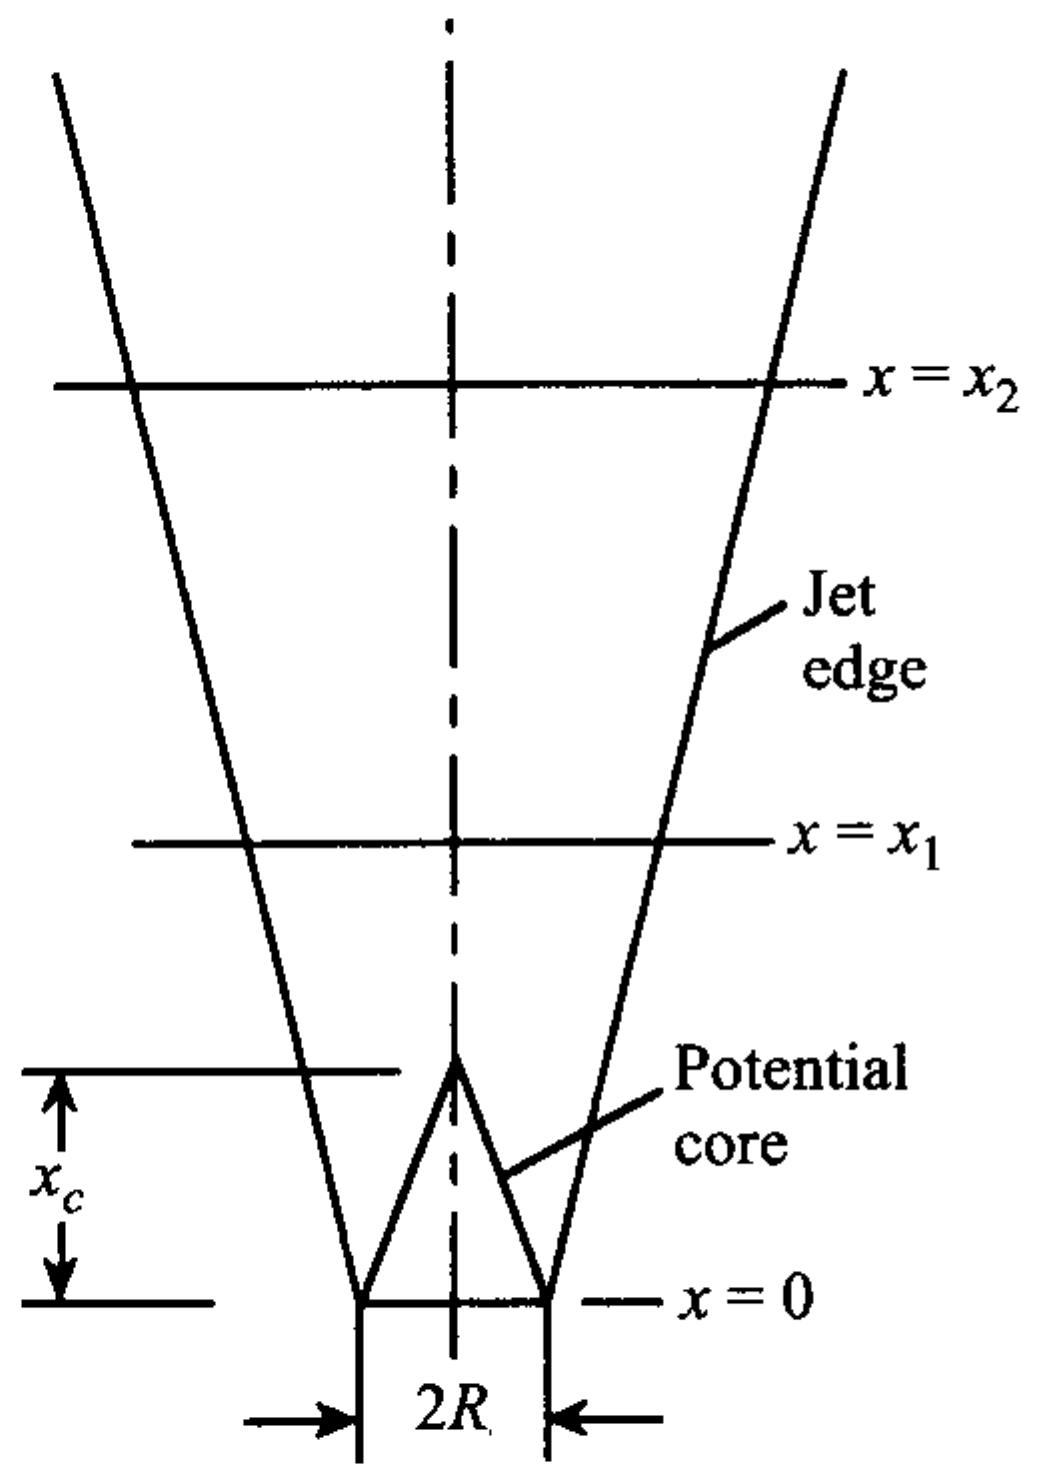
\includegraphics[width=0.6\linewidth]{jet}
				%\caption{}
				\label{fig:jet}
			\end{figure}
			\begin{align*}
			&J_e = \rho_e v_e^2 \pi R^2 \;\;;\;\; l_m = 0,075 \; \delta_{99\%} \\
			&\xi = \left[ \dfrac{3 J_e}{16 \rho_e \pi} \right] \dfrac{1}{\nu_t}\dfrac{r}{x} \\
			&\delta_{99\%} \rightarrow \text{raio no qual } \frac{\m{v}_x(r)}{\m{v}_{x,0}} = 1\%
			\end{align*}
		\end{column}
		\begin{column}{0.5\textwidth}
			\begin{figure}
				\centering
				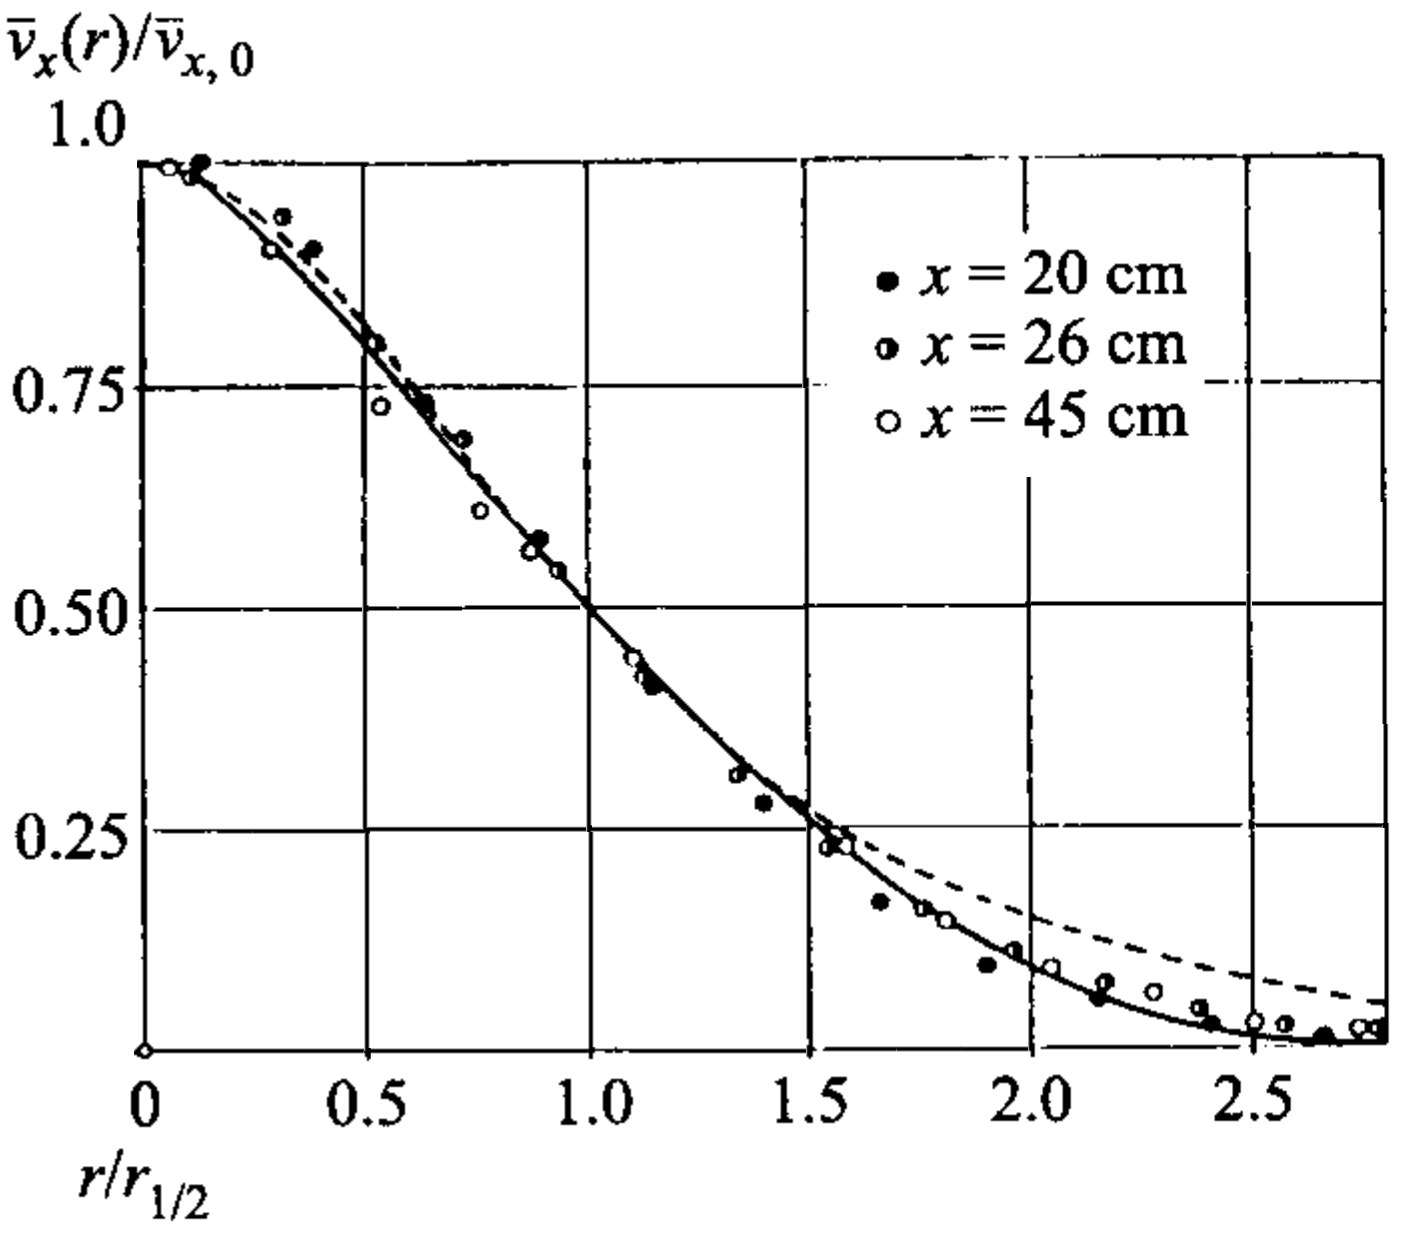
\includegraphics[width=0.9\linewidth]{jetVel}
				%\caption{}
				\label{fig:jetvel}
			\end{figure}
			\begin{enumerate}[a)]
				\item $\nu_t = 0,0102 \; \delta_{99\%} \; \m{v}_{x,0}(x) \approx cte$
				\item $r_{1/2} \propto x$ \\ $\m{v}_{x,0} \propto x^{-1}$
			\end{enumerate}

		\end{column}
	\end{columns}
\end{frame}

\begin{frame}{Eddy viscosity ou hipótese de Boussinessq (1877)}
	Aplicando a solução analítica p/ jato laminar:
	\begin{align*}
	&\mu_{lam} \Rightarrow \rho \nu_t \\
	&\m{v}_x = \dfrac{3}{8 \pi} \dfrac{J_e}{\rho \nu_t x}\left[ 1 + \dfrac{\xi^2}{4} \right]^{-2}
	\;\;\;\;\;\;\;\;
	\m{v}_r = \left[ \dfrac{3 J_e}{16 \pi \rho_e} \right]^{1/2} \dfrac{1}{x}\dfrac{\xi - \xi^3/4}{[1 + \xi^2/4]^2}
	\end{align*}
	
	Fazendo $ \dfrac{\m{v}_x}{v_e} = 0,375 (v_e R/\nu_t)(x/R)^{-1}[1 + \xi^2/4]^{-2} $, no centro $ r = 0 \Rightarrow \xi = 0 $
	
	\begin{align}
		 &\dfrac{\m{v}_x}{v_e} = 0,375 (v_e R/\nu_t)(x/R)^{-1}[1 + \xi^2/4]^{-2} \label{eq:vxve}\\
		 &\dfrac{\m{v}_x}{\m{v}_{x,0}} = \dfrac{1}{2} = \left[ 1 + \xi^2/4 \right]^{-2}
		 \rightarrow \xi = 1,287 = \dfrac{3}{16}\left[ \dfrac{\rho_e v_e^2 \pi R^2}{\rho_e \pi} \right]^{1/2}\dfrac{1}{\nu_t}\dfrac{r_{1/2}}{x} \nonumber \\
		 &\rightarrow 1,287 = 0,43 v_e R \dfrac{1}{\nu_t}\dfrac{r_{1/2}}{x} 
		 \rightarrow r_{1/2} = 2,97 \left( \dfrac{v_e R}{\nu_t x} \right)^{-1}\label{eq:r12}
	\end{align}
	
\end{frame}


\begin{frame}{Eddy viscosity ou hipótese de Boussinessq (1877)}
	Resolvendo \ref{eq:vxve}, \ref{eq:r12} e a)
	
	\begin{align*}
	&\dfrac{\m{v}_{x,o}}{v_e} = 13,15 (x/R)^{-1} \;\;\;\;\;\; \nu_t = 0,0285 v_e R \\
	& \dfrac{r_{1/2}}{x} = 0,08468
	\end{align*}
	
	Lembrando no caso laminar $ \dfrac{\m{v}_{x,0}}{v_e} \propto Re_{jet} $ e $ \dfrac{r_{1/2}}{x} \propto Re_{jet}^{-1}$. Portanto no caso turbulento existe independência do número de Reynolds.
\end{frame}

\begin{frame}{Equação de transporte p/ $ -\rho \m{u'_i u'_j} $}
	\begin{block}{Quantidade de movimento instantânea}
		\begin{equation}\label{eq:qtdMovInst}
		\ddxp{\rho u_i u_j}{j} = - \ddx{p}{i} + \ddx{\uptau_{ij}}{j}
		\end{equation}
	\end{block}

	Aplicando decomposição de Reynolds e a média temporal
	\begin{equation*}
	\dfrac{1}{\Delta t} \int_{0}^{t} \left[ \ddx{ }{j} \rho (\m{u}_i\m{u}_j + \m{u}_i u'_j + u'_i\m{u}_j + u'_i u'_j ) = -\ddxp{\m{p} + p'}{i} + \ddxp{\m{\uptau}_{ij} + \uptau'_{ij}}{j} \right] dt
	\end{equation*}
	\begin{equation*}
	\ddx{ }{j} \rho (\m{u}_i\m{u}_j + \m{u'_i u'_j}) = - \ddx{\m{p}}{i} + \ddx{\m{\uptau}_{ij}}{j}
	\end{equation*}

	\begin{block}{Quantidade de movimento média}
	\begin{equation}\label{eq:qtdMovMean}
	\ddxp{\rho \m{u}_i\m{u}_j}{j} = - \ddx{\m{p}}{i} + \ddxp{\m{\uptau}_{ij} - \rho \m{u'_i u'_j}}{j}
	\end{equation}
	\end{block}
	
\end{frame}


\begin{frame}{Equação de transporte p/ $ -\rho \m{u'_i u'_j} $}
	Reescrevendo o indice repetido como $k$ na equação \ref{eq:qtdMovInst} e multiplicando por $ \m{u}_i $ e $ \m{u}_j $ e somando as duas, lembrando a continuidade $ \ddxp{\rho u_i}{i} = 0 $ , temos para o termo advectivo
	\begin{align*}
	u_j \ddxp{\rho u_i u_k}{k} + u_i \ddxp{\rho u_j u_k}{k} \rightarrow 
	&\;\;\;\; u_j \left[ u_i \underbrace{\ddxp{\rho u_k}{k}}_{=0} + \rho u_k\ddx{u_i}{k}\right] \\
	&+ u_i \left[ u_j \underbrace{\ddxp{\rho u_k}{k}}_{=0} + \rho u_k\ddx{u_j}{k}\right]
	\end{align*}
	
	\begin{equation*}
	\rightarrow \rho u_j u_k \ddx{u_i}{k} + \rho u_i u_k \ddx{u_j}{k} \rightarrow \rho u_k \left[ u_j \ddx{u_i}{k} + u_i \ddx{u_j}{k} \right]
	\end{equation*}
	\begin{equation*}
	\rightarrow \rho u_k \ddxp{u_i u_j}{k} \rightarrow \boxed{\ddxp{\rho u_i u_j u_k}{k}}
	= \rho u_k \ddxp{u_i u_j}{k} + \rho u_i u_j \underbrace{\ddx{u_k}{k}}_{=0}
	\end{equation*}
\end{frame}

\begin{frame}{Equação de transporte p/ $ -\rho \m{u'_i u'_j} $}
	Assim a nova equação resulta
	
	\begin{equation*}
	\ddxp{\rho u_i u_j u_k}{k} = - u_j \ddx{p}{i} - u_i \ddx{p}{j} + u_j \ddx{\uptau_{ik}}{k} + u_i \ddx{\uptau_{jk}}{k}
	\end{equation*}
	
	Decomposição de Reynolds
	\begin{align*}
	\ddx{ }{k}\left[ \rho (\m{u}_i + u'_i) (\m{u}_j + u'_j) (\m{u}_k + u'_k) \right] = 
	&- (\m{u}_j + u'_j)\ddx{(\m{p} + p')}{i} \\ 
	&- (\m{u}_i + u'_i)\ddx{(\m{p} + p')}{j} \\
	&+ (\m{u}_j + u'_j) \ddxp{\m{\uptau}_{ik} + \uptau'_{ik}}{k} \\ 
	&+ (\m{u}_i + u'_i) \ddxp{\m{\uptau}_{jk} + \uptau'_{jk}}{k}
	\end{align*}
	
\end{frame}

\begin{frame}{Equação de transporte p/ $ -\rho \m{u'_i u'_j} $}
	Organizando e aplicando a média
	
	\begin{align*}
	\ddx{ }{k}\left[ \m{\rho \m{u}_i \m{u}_j} \m{u}_k + \m{\m{u}_i \rho u'_j u'_k} + \m{\m{u}_j \rho u'_i u'_k} + \m{\m{u}_k \rho u'_i u'_j} + \m{\rho u'_i u'_j u'_k} \right] \\
	=
	- \m{\m{u}_j \ddx{\m{p}}{i}} \red{- \m{\m{u}_j \ddx{p'}{i}} - \m{u'_j \ddx{\m{p}}{i}}} - \m{u'_j \ddx{p'}{i}}
	- \m{\m{u}_i \ddx{\m{p}}{j}} \red{- \m{\m{u}_i \ddx{p'}{j}} - \m{u'_i \ddx{\m{p}}{j}}} - \m{u'_i \ddx{p'}{j}} \\
	- \m{\m{u}_j \ddx{\m{\uptau}_{ik}}{k}} \red{- \m{\m{u}_j \ddx{\uptau'_{ik}}{k}} - \m{u'_j \ddx{\m{\uptau}_{ik}}{k}}} - \m{u'_j \ddx{\uptau'_{ik}}{k}}
	- \m{\m{u}_i \ddx{\m{\uptau}_{jk}}{k}} \red{- \m{\m{u}_i \ddx{\uptau'_{jk}}{k}} - \m{u'_i \ddx{\m{\uptau}_{jk}}{k}}} - \m{u'_i \ddx{\uptau'_{jk}}{k}}
	\end{align*}
	\begin{align}\label{eq:RSMinst}
	\ddx{ }{k}[ \rho \m{u}_i \m{u}_j \m{u}_k + \overbrace{\rho \m{u}_i \m{u'_j u'_k}}^{\incircle{A}} + \rho \overbrace{\m{u}_j \m{u'_i u'_k}}^{\incircle{B}} + \rho \m{u}_k \m{u'_i u'_j} + \rho \m{u'_i u'_j u'_k} ] \nonumber \\
	=
	- \m{u}_j \ddx{\m{p}}{i} - \m{u'_j \ddx{p'}{i}}
	- \m{u}_i \ddx{\m{p}}{j} - \m{u'_i \ddx{p'}{j}}
	- \m{u}_j \ddx{\m{\uptau}_{ik}}{k} - \m{u'_j \ddx{\uptau'_{ik}}{k}}
	- \m{u}_i \ddx{\m{\uptau}_{jk}}{k} - \m{u'_i \ddx{\uptau'_{jk}}{k}}
	\end{align}
\end{frame}

\begin{frame}{Equação de transporte p/ $ -\rho \m{u'_i u'_j} $}
	Reescrevendo o indice repetido como $k$ na equação \ref{eq:qtdMovMean} e multiplicando por $ \m{u}_i $ e por $ \m{u}_j $ e então somando as duas equações resultantes temos
	\begin{equation}\label{eq:RSMmean}
	\ddxp{\rho \m{u}_i \m{u}_j \m{u}_k}{k} = - \m{u}_j \ddx{\m{p}}{i} - \m{u}_i \ddx{\m{p}}{j} + \m{u}_j \ddx{}{k}(\m{\uptau}_{ik} - \overbrace{\rho\m{u'_iu'_k}}^{\incircle{B'}}) + \m{u}_i \ddx{}{k}(\m{\uptau}_{jk} - \overbrace{\rho\m{u'_ju'_k}}^{\incircle{A'}})
	\end{equation}
	
	Subtraindo \ref{eq:RSMmean} de \ref{eq:RSMinst}, sendo $\incircle{A} = \incircle{A'} - \rho \m{u'_ju'_k}\ddx{\m{u}_i}{k}$, e similar $\incircle{B} $ e $ \incircle{B'} $
	
	\begin{block}{Equação de transporte de $ \m{u'_i u'_j} $}
		\begin{align}\label{eq:uiuj}
	\ddxp{\rho \m{u}_k \m{u'_i u'_j}}{k} = &- \ddxp{\rho \m{u'_iu'_ju'_k}}{k} - \m{u'_j\ddx{p'}{i}} - \m{u'_i\ddx{p'}{j}} \nonumber \\
	&+ \m{u'_j\ddx{\uptau'_{ik}}{k}} + \m{u'_i\ddx{\uptau'_{jk}}{k}}
	- \rho \m{u'_i u'_k} \ddx{\m{u}_i}{k} - \rho \m{u'_j u'_k} \ddx{\m{u}_j}{k} 
	\end{align}
	\end{block}
		
\end{frame}

\begin{frame}{Equação de transporte p/ $ -\rho \m{u'_i u'_j} $}
	
	\begin{enumerate}[$\bullet$]
		\item Termos de tensões:
	\end{enumerate}
	
	\begin{equation*}
	\m{u'_j\ddx{\uptau'_{ik}}{k}} + \m{u'_i\ddx{\uptau'_{jk}}{k}} \;\;;\;\; \uptau'_{ik} = \mu \ddx{u'_i}{k}
	\end{equation*}
	\begin{align*}
	&\rightarrow \m{u'_j\ddxp{\mu \ddx{u'_i}{k}}{k}} + \m{u'_i\ddxp{\mu \ddx{u'_j}{k}}{k}} \\
	&\rightarrow \mu \left[ \ddxp{\m{u'_j \ddx{u'_i}{k}}}{k} - \m{\ddx{u'_i}{k}\ddx{u'_j}{k}} + \ddxp{\m{u'_i \ddx{u'_j}{k}}}{k} - \m{\ddx{u'_i}{k}\ddx{u'_j}{k}} \right] \\
	&\rightarrow \mu \left[ \ddxp{\ddx{(\m{u'_iu'_j})}{k}}{k} - 2 \m{\ddx{u'_i}{k}\ddx{u'_j}{k}} \right]
	\end{align*}
	
	\begin{enumerate}[$\bullet$]
		\item Termo de dissipação:
	\end{enumerate}
	\begin{equation*}
	\mu \m{\ddx{u'_i}{k}\ddx{u'_j}{k}} = \varepsilon_{ik} = \dfrac{2}{3} \delta_{ik}\varepsilon
	\end{equation*}
	
	
\end{frame}

\begin{frame}{Equação de transporte p/ $ -\rho \m{u'_i u'_j} $}
	\begin{enumerate}[$\bullet$]
		\item Termos de pressão:
	\end{enumerate}

	\begin{align*}
	- \m{u'_j\ddx{p'}{i}} - \m{u'_i\ddx{p'}{j}} 
	&\rightarrow - \ddxp{\m{p' \delta_{ki} u'_j}}{k} + \m{p'\ddx{u'_j}{i}} - \ddxp{\m{p' \delta_{kj} u'_i}}{k} + \m{p'\ddx{u'_i}{j}} \\
	&\rightarrow - \ddxp{\m{p' \delta_{ki} u'_j} + \m{p' \delta_{kj} u'_i}}{k} + \m{p'\left( \ddx{u'_j}{i} + \ddx{u'_i}{j} \right)}
	\end{align*}

\end{frame}

\begin{frame}{Equação de transporte p/ $ -\rho \m{u'_i u'_j} $}
	Finalmente temos
	
	\begin{block}{Equação de transporte de $ \m{u'_i u'_j} $}
		\begin{align}\label{eq:uiujfinal}
		\ddxp{\rho \m{u}_k \m{u'_i u'_j}}{k} = &- \ddxp{\rho \m{u'_iu'_ju'_k}}{k} - \ddxp{\m{p' \delta_{ki} u'_j} + \m{p' \delta_{kj} u'_i}}{k} \nonumber \\
		&+ \m{p'\left( \ddx{u'_j}{i} + \ddx{u'_i}{j} \right)} + \mu \left[ \ddxp{\ddx{(\m{u'_iu'_j})}{k}}{k} \right] \nonumber \\
		&- \dfrac{2}{3} \delta_{ik}\varepsilon
		- \rho \m{u'_i u'_k} \ddx{\m{u}_i}{k} - \rho \m{u'_j u'_k} \ddx{\m{u}_j}{k} 
		\end{align}
	\end{block}
	
	A partir da equação \ref{eq:uiujfinal}, chegar na equação da energia cinética turbulenta $ K = \left( \dfrac{1}{2} \m{u'_i u'_i} \right) $.
	
\end{frame}

\begin{frame}[b]{Considerações finais}
	\vfill
	\begin{beamercolorbox}[wd=\textwidth,rounded=true,shadow=true]{block body example}
		\vfill
		\centering \textbf{Perguntas?}
		\vspace*{10pt}
	\end{beamercolorbox}
	\vfill
	\doclicenseThis
\end{frame}

\end{document}